%%%%%%%%%%%%%%%%%%%%%%%%%%%%%%%%%%%%%%%%%%%%%%%%%%%%%%%%%%%%%%%%%%%%%%%%%%%%%%%%%%%%
% Document data
%%%%%%%%%%%%%%%%%%%%%%%%%%%%%%%%%%%%%%%%%%%%%%%%%%%%%%%%%%%%%%%%%%%%%%%%%%%%%%%%%%%%
\documentclass[12pt]{article}
%%%%%%%%%%%%%%%%%%%%%%%%%%%%%%%%%%%%%%%%%%%%%%%%%%%%%%%%%%%%%%%%%%%%%%%%%%%%%%%%%%%%




%%%%%%%%%%%%%%%%%%%%%%%%%%%%%%%%%%%%%%%%%%%%%%%%%%%%%%%%%%%%%%%%%%%%%%%%%%%%%%%%%%%%
% Packages
%%%%%%%%%%%%%%%%%%%%%%%%%%%%%%%%%%%%%%%%%%%%%%%%%%%%%%%%%%%%%%%%%%%%%%%%%%%%%%%%%%%%
\usepackage{color, soul, xcolor} % Colored text and highlighting, respectively
\usepackage{tikz-cd} % For commutative diagrams
\usepackage{mathtools}
\usepackage{answers}
\usepackage{setspace}
\usepackage{graphicx}
\usepackage{enumerate}
\usepackage{multicol}
\usepackage{mathrsfs}
\usepackage[margin=.75in]{geometry} 
\usepackage{amsmath,amsthm,amssymb}
\usepackage{marvosym,wasysym} %fucking smileys
%%%%%%%%%%%%%%%%%%%%%%%%%%%%%%%%%%%%%%%%%%%%%%%%%%%%%%%%%%%%%%%%%%%%%%%%%%%%%%%%%%%%




%%%%%%%%%%%%%%%%%%%%%%%%%%%%%%%%%%%%%%%%%%%%%%%%%%%%%%%%%%%%%%%%%%%%%%%%%%%%%%%%%%%%
% Shortcuts
%%%%%%%%%%%%%%%%%%%%%%%%%%%%%%%%%%%%%%%%%%%%%%%%%%%%%%%%%%%%%%%%%%%%%%%%%%%%%%%%%%%%
% Number systems
\newcommand{\N}{\mathbb{N}}
\newcommand{\Z}{\mathbb{Z}}
\newcommand{\C}{\mathbb{C}}
\newcommand{\R}{\mathbb{R}}
\newcommand{\Q}{\mathbb{Q}}

% Operators/functions
\newcommand{\id}{\mathrm{Id}}
\DeclareMathOperator{\sech}{sech}
\DeclareMathOperator{\csch}{csch}
%%%%%%%%%%%%%%%%%%%%%%%%%%%%%%%%%%%%%%%%%%%%%%%%%%%%%%%%%%%%%%%%%%%%%%%%%%%%%%%%%%%%




%%%%%%%%%%%%%%%%%%%%%%%%%%%%%%%%%%%%%%%%%%%%%%%%%%%%%%%%%%%%%%%%%%%%%%%%%%%%%%%%%%%%
% Environments
%%%%%%%%%%%%%%%%%%%%%%%%%%%%%%%%%%%%%%%%%%%%%%%%%%%%%%%%%%%%%%%%%%%%%%%%%%%%%%%%%%%%
% Italic font
\newtheorem{theorem}{Theorem}[section]
\newtheorem{lemma}{Lemma}[section]
\newtheorem{corollary}{Corollary}[section]

% Plain font
\theoremstyle{definition}
\newtheorem{definition}{Definition}[subsection]
\newtheorem{definitions}{Definitions}[subsection]
\newtheorem{example}{Example}[subsection]
\newtheorem{remark}{Remark}[subsection]
\newtheorem{solution}{Solution}[subsection]
\newtheorem{problem}{Problem}[subsection]
\newtheorem{answer}{Answer}[subsection]
\newtheorem{question}{Question}
\newtheorem{exercise}{Exercise}[subsection]
%%%%%%%%%%%%%%%%%%%%%%%%%%%%%%%%%%%%%%%%%%%%%%%%%%%%%%%%%%%%%%%%%%%%%%%%%%%%%%%%%%%%
 
 
 
%%%%%%%%%%%%%%%%%%%%%%%%%%%%%%%%%%%%%%%%%%%%%%%%%%%%%%%%%%%%%%%%%%%%%%%%%%%%%%%%%%%%
% Beginning of document
%%%%%%%%%%%%%%%%%%%%%%%%%%%%%%%%%%%%%%%%%%%%%%%%%%%%%%%%%%%%%%%%%%%%%%%%%%%%%%%%%%%%
\begin{document}
\noindent
\LARGE\textbf{Post Test} \hfill \textbf{Name:~\underline{~~~~~~~~~~~~~~~~~~~}}\\

\normalsize
\begin{question}[Derivative Rules] Let $f,g,h$ be sufficiently smooth (differentiable) functions of $x$ with agreeable domains and ranges.  
    \begin{enumerate}[(a)]
        \item Recall $(h\circ g \circ f)(x)=h(g(f(x)))$. What is $(h\circ g \circ f)'(x)?$ (Apply the chain rule to three functions.)
        \item What is $(fgh)'(x)=\frac{d}{dx}(f(x)\cdot g(x)\cdot h(x))?$ (Apply the product rule to three functions.)
        \item Evaluate $\frac{d}{dx} \left( \frac{\sin (x^2+x)}{x}+e^x\right).$
    \end{enumerate}
\end{question}

\pagebreak




\begin{question}[Interpreting the Derivative]
Take the following graph of the time derivative of the position function (velocity) for $x'(t)$ versus time $t$ for some object.\\

\begin{figure}[h]
    \centering
    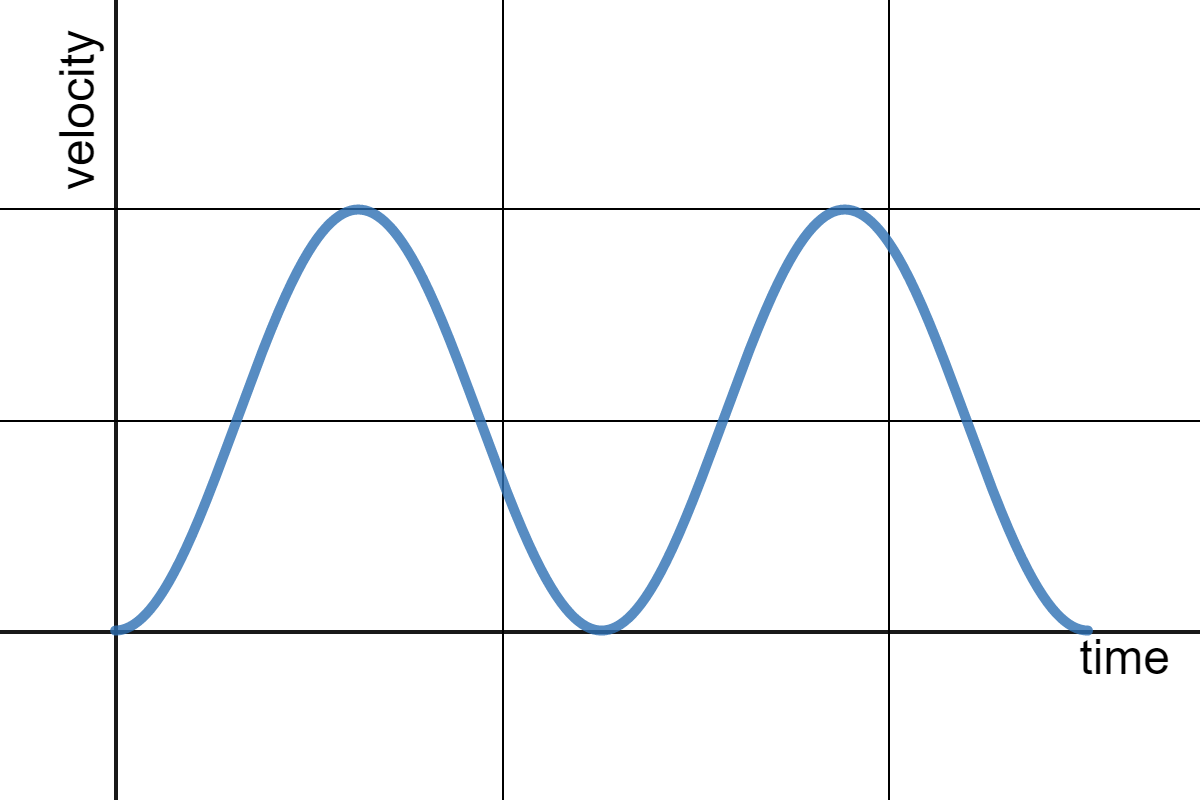
\includegraphics[scale=.2]{desmos-graph.png}
    \caption{Velocity $x'(t)$ versus time $t$. Note that $x'(0)=0.$}
    \label{fig:my_label}
\end{figure}
\begin{enumerate}[(a)]
    \item Provide a situation in which this graph describes a velocity (Hint: Driving a car.)
    \item Label the points where the object moving the fastest.
    \item Does the object ever move backwards?
    \item How could you find the total distance the object moved?
    \item Draw the derivative of this graph.
\end{enumerate}
\end{question}

\pagebreak





\begin{question}[Small Angle Approximation]
Recall that we have the Taylor series representation for $\sin x$ given by
\[
\sin x = \sum_{n=0}^\infty \frac{(-1)^n x^{2n+1}}{(2n+1)!}.
\]
\begin{enumerate}[(a)]
    \item What is the leading order term in the series?
    \item For roughly how large of an angle is this leading order approximation reasonable?
\end{enumerate}
\end{question}

\pagebreak




\begin{question}[Integration] Consider the following: 
\[
I(x)=\int_{x_0}^x \tilde{x} e^{\tilde{x}} d\tilde{x}
\]
\begin{enumerate}[(a)]
    \item Evaluate the definite integral.
    \item Given $I(0)=0$ find $x_0$. 
\end{enumerate}
\end{question}

\pagebreak



\begin{question}[Interpeting the Integral]
Take the following graph of the second time derivative of the position function (acceleration) for $x''(t)$ versus time $t$ for some object.\\

\begin{figure}[h]
    \centering
    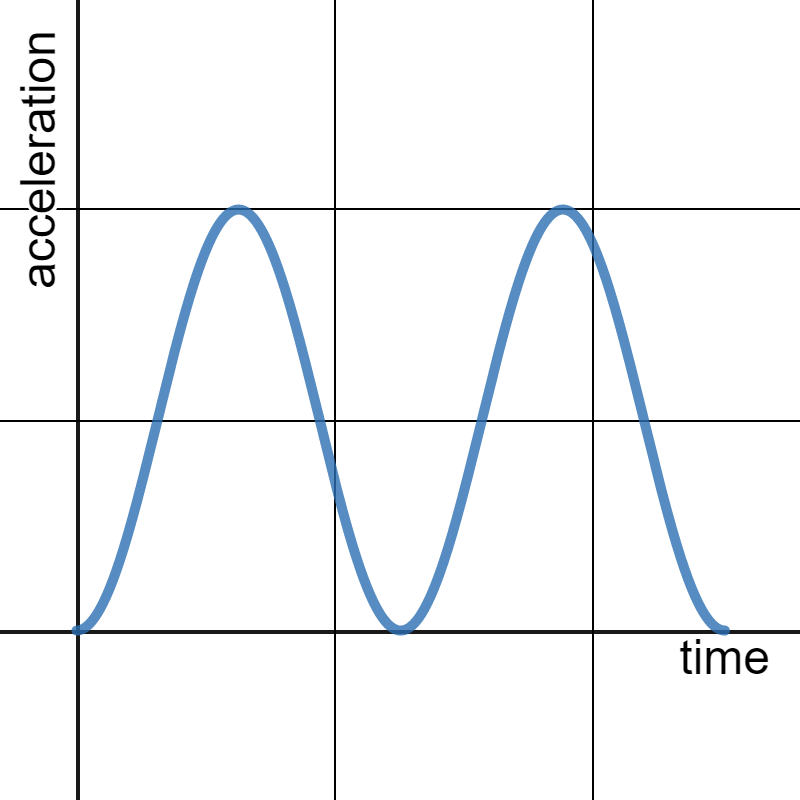
\includegraphics[scale=.2]{acceleration.png}
    \caption{Acceleration $x''(t)$ versus time $t$. Note that $x''(0)=0.$}
    \label{fig:my_label}
\end{figure}
\begin{enumerate}[(a)]
    \item What function do we get when we take the indefinite integral once? Is this new function determined uniquely? Why or why not?
    \item Knowing the mass $m$ of the object and that it is at rest at time $t=0$, we can integrate
    \[
    I=\int_0^{t_f} mx''(t)dt,
    \]
    which is the impulse (change in momentum) of the object. After applying this impulse, is the object moving faster, slower, or the same?
\end{enumerate}
\end{question}


\end{document}